% TikZ code for K^(2)(2, 2, 2) using predefined edge colors
\pgfdeclarelayer{background}
\pgfdeclarelayer{main}
\pgfsetlayers{background,main}
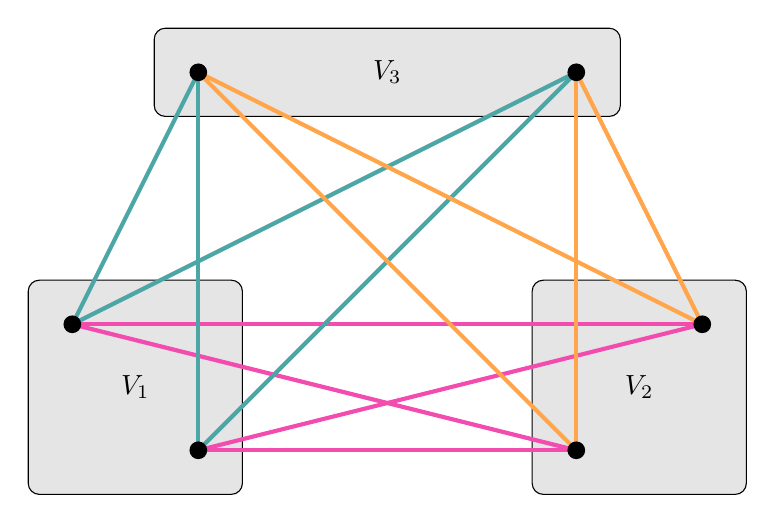
\begin{tikzpicture}[scale=0.8]
\begin{pgfonlayer}{background}
  \draw[fill=gray!20, rounded corners] (-0.70, -0.70) rectangle (2.70, 2.70);
\end{pgfonlayer}
\node at (1.00, 1.00) [align=center] {$V_1$};
\begin{pgfonlayer}{background}
  \draw[fill=gray!20, rounded corners] (7.30, -0.70) rectangle (10.70, 2.70);
\end{pgfonlayer}
\node at (9.00, 1.00) [align=center] {$V_2$};
\begin{pgfonlayer}{background}
  \draw[fill=gray!20, rounded corners] (1.30, 5.30) rectangle (8.70, 6.70);
\end{pgfonlayer}
\node at (5.00, 6.00) [align=center] {$V_3$};
\coordinate (A1) at (2, 0);
\coordinate (A2) at (0, 2);
\coordinate (B1) at (8, 0);
\coordinate (B2) at (10, 2);
\coordinate (C1) at (2, 6);
\coordinate (C2) at (8, 6);
\draw[line width=1.5pt, color=magenta!70!white] (A1) -- (B1);
\draw[line width=1.5pt, color=magenta!70!white] (A1) -- (B2);
\draw[line width=1.5pt, color=magenta!70!white] (A2) -- (B1);
\draw[line width=1.5pt, color=magenta!70!white] (A2) -- (B2);
\draw[line width=1.5pt, color=teal!70!white] (A1) -- (C1);
\draw[line width=1.5pt, color=teal!70!white] (A1) -- (C2);
\draw[line width=1.5pt, color=teal!70!white] (A2) -- (C1);
\draw[line width=1.5pt, color=teal!70!white] (A2) -- (C2);
\draw[line width=1.5pt, color=orange!70!white] (B1) -- (C1);
\draw[line width=1.5pt, color=orange!70!white] (B1) -- (C2);
\draw[line width=1.5pt, color=orange!70!white] (B2) -- (C1);
\draw[line width=1.5pt, color=orange!70!white] (B2) -- (C2);
\begin{pgfonlayer}{main}
  \fill[black] (A1) circle (4.0pt);
  \fill[black] (A2) circle (4.0pt);
  \fill[black] (B1) circle (4.0pt);
  \fill[black] (B2) circle (4.0pt);
  \fill[black] (C1) circle (4.0pt);
  \fill[black] (C2) circle (4.0pt);
\end{pgfonlayer}
\end{tikzpicture}